\item \points{18} {\bf Constructing kernels}

In class, we saw that by choosing a kernel $K(x,z) = \phi(x)^T\phi(z)$, we can
implicitly map data to a high dimensional space, and have a learning algorithm (e.g SVM or logistic regression)
work in that space. One way to generate kernels is to explicitly define the
mapping $\phi$ to a higher dimensional space, and then work out the
corresponding $K$.

However in this question we are interested in direct construction of kernels.
I.e., suppose we have a function $K(x,z)$ that we think gives an appropriate
similarity measure for our learning problem, and we are considering plugging
$K$ into the SVM as the kernel function. However for $K(x,z)$ to be a valid
kernel, it must correspond to an inner product in some higher dimensional space
resulting from some feature mapping $\phi$.  Mercer's theorem tells us that
$K(x,z)$ is a (Mercer) kernel if and only if for any finite set $\{x^{(1)},
\ldots, x^{(\nexp)}\}$, the square matrix $K \in \Re^{\nexp \times \nexp}$ whose entries
are given by $K_{ij} = K(x^{(i)},x^{(j)})$ is symmetric and positive
semidefinite. You can find more details about Mercer's theorem in the notes,
though the description above is sufficient for this problem.

Now here comes the question: Let $K_1$, $K_2$ be kernels over $\Re^{\di} \times
\Re^{\di}$, let $a \in \Re^+$ be a positive real number, let $f : \Re^{\di} \mapsto
\Re$ be a real-valued function, let $\phi: \Re^{\di} \rightarrow \Re^\nf$ be a
function mapping from $\Re^{\di}$ to $\Re^\nf$, let $K_3$ be a kernel over $\Re^\nf
\times \Re^\nf$, and let $p(x)$ a polynomial over $x$ with \emph{positive}
coefficients.

For each of the functions $K$ below, state whether it is necessarily a
kernel.  If you think it is, prove it; if you think it isn't, give a
counter-example.

\begin{enumerate}

\item \subquestionpoints{1} $K(x,z) = K_1(x,z) + K_2(x,z)$
\item \subquestionpoints{1} $K(x,z) = K_1(x,z) - K_2(x,z)$
\item \subquestionpoints{1} $K(x,z) = a K_1(x,z)$
\item \subquestionpoints{1} $K(x,z) = -a K_1(x,z)$
\item \subquestionpoints{5} $K(x,z) = K_1(x,z)K_2(x,z)$
\item \subquestionpoints{3} $K(x,z) = f(x)f(z)$
\item \subquestionpoints{3} $K(x,z) = K_3(\phi(x),\phi(z))$
\item \subquestionpoints{3} $K(x,z) = p(K_1(x,z))$

\end{enumerate}

[\textbf{Hint:} For part (e), the answer is that $K$ \emph{is} indeed
a kernel. You still have to prove it, though.  (This one may be harder than the
rest.)  This result may also be useful for another part of the problem.]

\ifnum\solutions=1 {
  \begin{answer}
After many trials, I found an instance where the algorithm is able to converge after 193 trials. 
\begin{figure}[here] %  figure placement: here, top, bottom, or page
   \centering
   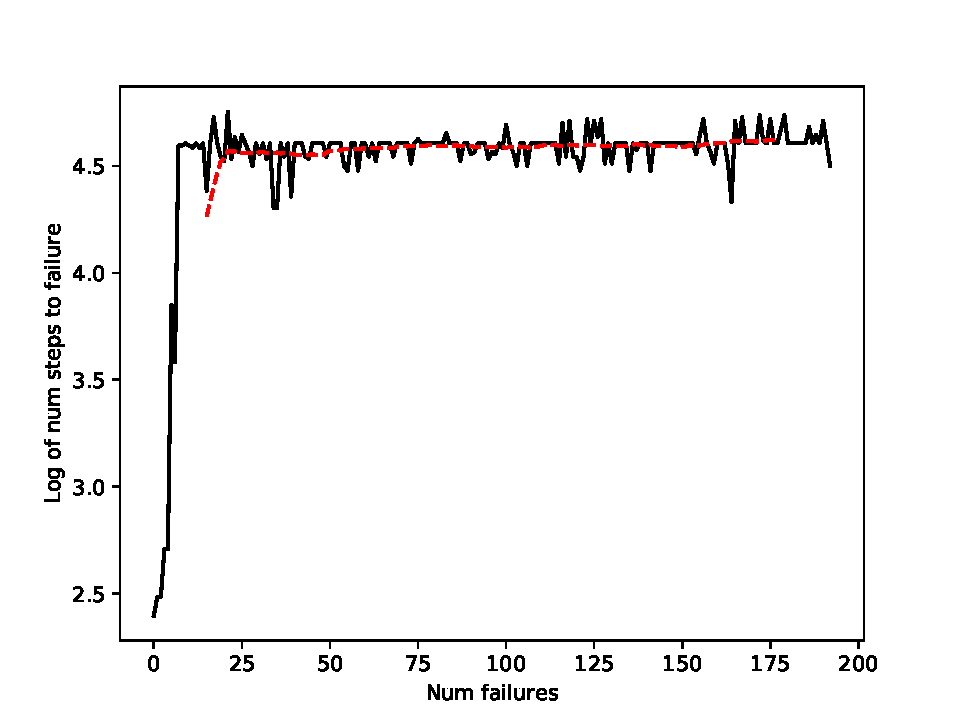
\includegraphics[width=6in]{control6.pdf} 
   \caption{Steps by Failures until Convergence}
   \label{fig:example}
\end{figure}
\end{answer}

} \fi
